\chapter{Background}
This chapter introduces the necessary background information needed for understanding the rest of the report.
First section, provides a broad introduction to \ac{sdr} systems, GNU Radio Software Tool and \ac{PHY} and \ac{mac} layers of the network stack.
The second section introduces previous work in this domain, which are critically analyzed to help concretely define the problem area.
Finally the last section, introduces the LimeSDR platform, IEEE 802.15.4 based system design and the tools used in the methods section.


\section{Essential Concepts}
\subsection{\ac{PHY} and \ac{mac} Layers}
\ac{OSI} Model (ISO/IEC 7498-1:1994) presents the abstract model for networking, that is used for most communication systems design.
The abstract model is divided into 7 layers,  where entity in each layer implements the functionality of the layer and interacts directly with the layer beneath it, the added functionality can be used by the upper layers.
Data from the user application is encapsulated by each subsequent layers of the \ac{OSI} model into their frame format.
These frames carry meta-data in the form of frame headers.
Different protocols use different frame format and headers  as it helps differentiate one protocol from another.
These headers help the receiver in learning where the incoming data packet is coming from, who is it meant for, how to decode and arrange the contents of the data packets etc.\\

\ac{PHY} layer is the lowest layer (L1) of the \ac{OSI} model,it interacts with the physical communication channel directly.
It defines the type of data transfer(serial/parallel) and data rate of the protocol.
\ac{PHY} layer defines the process of transmitting raw bits through the physical medium.
The bit-stream is grouped into code words and converted to symbols, which are then modulated to a physical signal for transmission over the transmission medium.
\ac{PHY} layers also provides physical transmission link information like carrier sense and collision detection and \ac{LQI}  to the upper layers. \\


\ac{mac} layer, \ac{L2} of the \ac{OSI} model, is responsible for defining the the methods for sharing and using the common transmission medium among multiple devices.
\ac{mac} layer addresses are used to to check if the incoming packet is meant for the device.
In case of outgoing packets, the \ac{mac} layer adds the \ac{mac} address of the destination device to the packet header.
It adds the synchronization preamble and \ac{FCS} for checking transmission error.
Retransmission in case of dropped packets and acknowledgement to successfully received packets are handled by this layer.\\

\begin{figure}[h!]
\centering
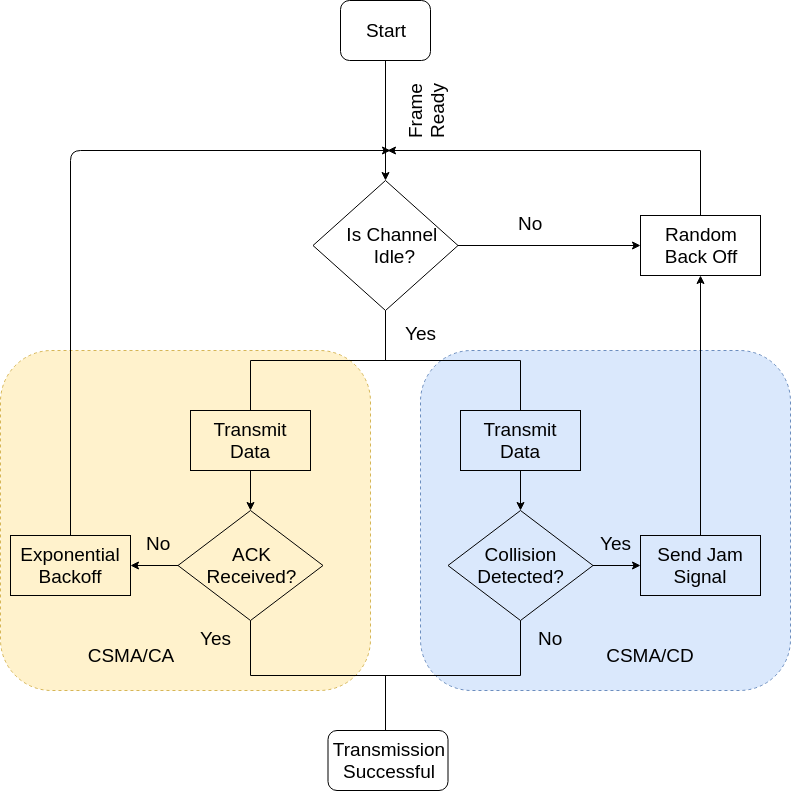
\includegraphics[width=0.9\textwidth]{Figure/CSMA.png}
\caption{CSMA flow graph.}
\label{Csma_flow}
\end{figure}

\ac{csma} is \ac{L2} protocol of the OSI Model. 
It is a method for handling multiple access of a shared medium.
It mainly comes in two varieties: \ac{CSMA/CD}  and \ac{CSMA/CA}. In the older \ac{CSMA/CD}, the nodes wait until the frame is ready, then check is the medium is idle or not.
If idle it starts transmission.
During transmission, it monitors the medium for collision.
If collision is detected, it employs a collision recovery process, where it sends a jam signal to signal other nodes that a collision has occurred.
Then it waits for a  random delay and starts transmission again.\\

\ac{CSMA/CA} tries to avoid collision, it starts off similar to \ac{CSMA/CD} where it senses to check when the channel is idle.
If found idle, it starts transmission.
As it is difficult for wireless nodes to detect collision at the same time its transmitting therefore it relies on an \ac{ack} from the receiving node to check if the data packet was received.
If \ac{ack} is not received, the node assumes a collision has occurred and  uses exponential back-off to determine when the next time to re initiate transmission.\\


\ac{tdma} is also a \ac{L2} protocol, where a coordinator schedules medium access to the nodes in a periodic manner.
Communication happens in time-slots.
Each node in the network is given exclusive access to transmit during its time slot.
The coordinator generates beacon signals periodically to maintain relative time synchronization. On receiving the beacons, the nodes adjust their transmit clocks so that they have the correct estimate of their time-slots.
 
 

\subsection{\ac{sdr} Platforms}

\ac{sdr} represents a new paradigm of communication system design where the system is flexible to adapt to the needs of the end-user as also the radio channel conditions. Nychis et.al \cite{nychis_enabling_nodate} classifies \ac{sdr} based communication systems into two main architectures.
\begin{itemize} 
\item{\textit{Host-PHY Architecture:} This is the most common architecture, enabling design and development of the entire system in software.
It provides the maximum flexibility in terms of design and implementation choices, also there is added benefit of easy upgrades.
But, since the system is designed is software only, the processing and communication delays make most modern \ac{mac} protocols infeasible in this architecture.}


\item{\textit{NIC-PHY Architecture:} In this architecture most of the \ac{PHY} layer functionality is implemented in \ac{FPGA} and \ac{DSP}.
The closer proximity to the radio hardware and specialized parallel hardware processing makes this architecture most suitable for running the modern \ac{mac} protocols.
But the design process for this architecture based systems is time consuming and difficult, as traditionally hardware programming harder simple software programming.
However, they are much more flexible compared to commercial \ac{NIC}.
\textit{Wireless Open Access Research Platform}(WARP) \cite{noauthor_warp_nodate} is an example of system based on this type of architecture.}

\end{itemize}
Since host-PHY \cite{nychis_enabling_nodate} is the most commonly used architecture (\textbf{cite sources}), the report concentrates on explaining the functionality of \ac{sdr} systems using this architecture.
Figure \ref{host_PHY} shows the typical design of communication systems in this architecture. The system can be broadly divided into two main components:
\begin{enumerate}
\item{\ac{sdr} Platform.}
\item{Host Computer.}
\end{enumerate}

\begin{figure}[h!]
\centering
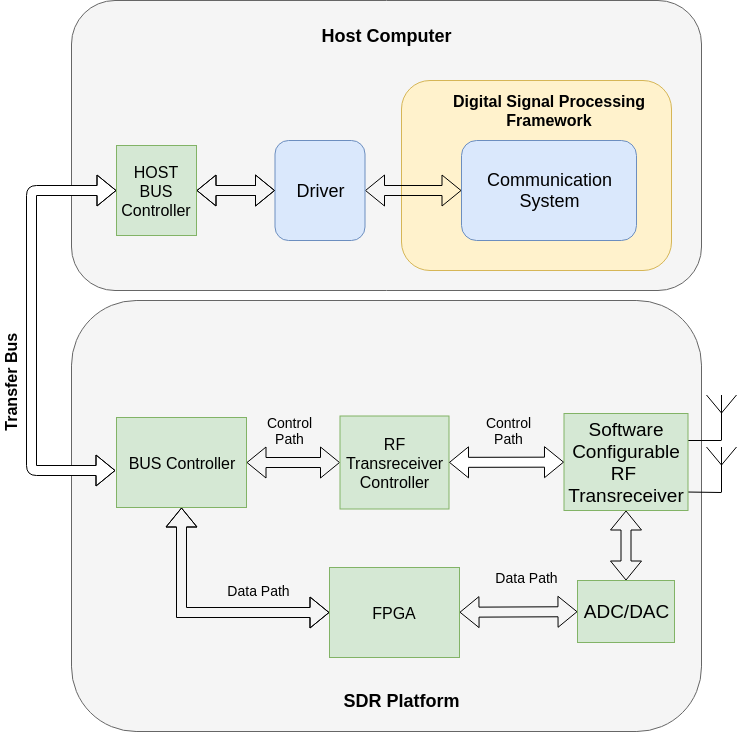
\includegraphics[width=\textwidth]{Figure/Host_Phy.png}
\caption{Host-PHY \cite{nychis_enabling_nodate} \ac{sdr} architecture.}
\label{host_PHY}
\end{figure}


Since the process for transmission and reception are symmetric, this report concentrates on the explaining the reception side of 
\ac{sdr} platforms.

\paragraph{\ac{sdr} Platform:} It is the hardware that provides access to the wireless medium in a flexible manner.
\ac{RF} signals are transmitted and received by the platform, it converts these analog signals to digital samples and transfers them to the host computer.
The main building blocks of these platforms are shown in \ref{host_PHY}.
\begin{itemize}
\item{\textbf{Software Configurable \ac{RF} trans-receiver}} This is the heart of \ac{sdr} platforms and provides \ac{RF} modulation and demodulation capability.
They are attached to wide-band antennas for receiving and transmitting over a broad range of frequencies.
Taking the case of reception of RF signal, the signal received from the antenna is amplified by a \ac{LNA}.
The \ac{LNA} amplifies a low power signal without significantly degrading the signal to noise ratio.
Once amplified, the signal to passed to a \ac{RF} receiver, where the \ac{RF} signal is demodulated either to a intermediate frequency or baseband signal depending on whether the the receiver is a Zero-IF receiver or Super-heterodyne receiver respectively.\\

\begin{figure}[h!]
\centering
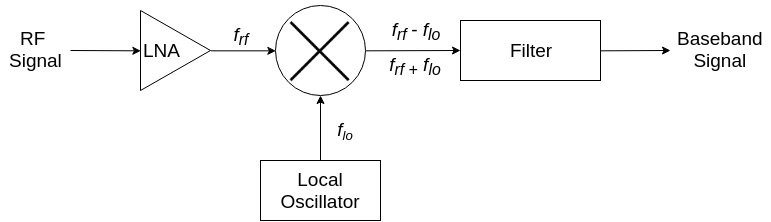
\includegraphics[width=0.8\textwidth]{Figure/RF_receiver.png}
\caption{Simple \ac{RF} receiver.}
\label{rf_receiver}
\end{figure}

Figure \ref{rf_receiver} shows a simple \ac{RF} receiver, the \ac{LNA} output signal is fed to a mixer.
The mixer is a signal processing block used for translating the input signal to another frequency range.
The mixer uses a locally generated carrier frequency for the translation. 
If the input \ac{RF} signal has a frequency of $f_{rf}$, and the local oscillator frequency is $f_{lo}$ then the mixer will produce a signal with frequency components $f_{rf}-f_{lo}$ and $f_{rf}+f_{lo}$.
This output signal is then passed through a band-pass filter with $f_{rf}-f_{lo}$ as center frequency, this will reject the unwanted $f_rf+f_lo$.
In the assume $f_{rf}=f_{lo}$, the bandpass filter will become a low pass filter and the output signal will be the baseband signal.
This is the case in Zero-IF receiver architecture.
In super heterodyne receiver architecture, a number of stages of intermediate frequency are used before generation of the baseband signal.\\

In traditional trans-receiver, a crystal oscillator is used.
This results in good stability of the local oscillator signal but the system is now tuned to a particular frequency.
With the goal of flexibility in mind, \ac{sdr} platforms use frequency synthesizers to generate the local clock signal.
Frequency synthesizers are used for creating arbitrary waveforms from a single frequency clock.
Most \ac{sdr} use \ac{DDS} as the frequency synthesizer, which uses a highly stable oscillator used as a reference signal.



\begin{figure}[h!]
\centering
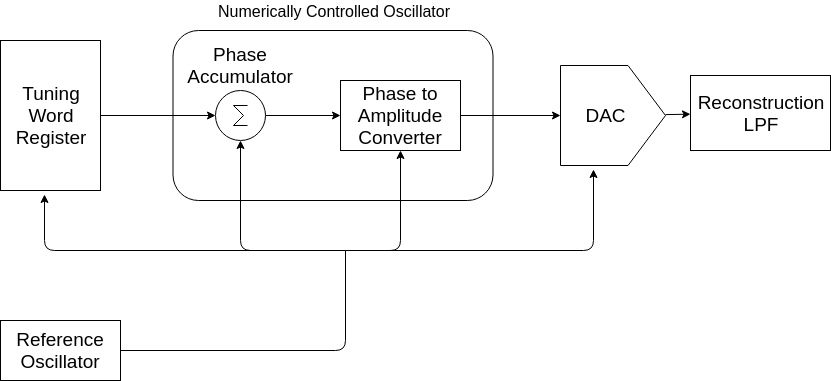
\includegraphics[width=0.8\textwidth]{Figure/DDS.png}
\caption{\ac{DDS}.}
\label{dds}
\end{figure}

The main components of a \ac{DDS} are \ac{NCO} which is made of the Phase Accumulator and Phase to Amplitude Converter, \ac{DAC} and a Tuning Word Register as shown in Figure \ref{dds}.

In each clock cycle, the phase accumulator increases the output by the value stored in the Tuning Word Register.
This output is the input to the Phase to Amplitude Converter, which basically is a lookup table containing the amplitude for a particular phase.
The output of the Phase Accumulator is basically the address(phase) for the lookup table.
The output is then converted to an analog signal by the the \ac{DAC} and then passed through a low pass filter to smoothen out the waveform.

Since the Tuning Word Register is responsible for how fast the phase changes, the output sinusoid frequency can be controlled by controlling the Tuning Word Register, this is how \ac{sdr} platforms are able to generate a wide range of local oscillator frequencies.

In \ac{sdr} platforms, the filter is implemented using \ac{FIR} filters.
\ac{FIR} filters are convolutional filters where the output response of a particular input is finite.
The output of a \ac{FIR} filter can be adjusted by readjusting the parameters of the filter's impulse response.
This allows for the \ac{sdr} to allow certain range of frequencies in the output, which can be adjusted by external control.

\item{\textbf{\ac{RF} Trans receiver Controller:} The controller provides the interface to control the \ac{RF} Transceiver.
The communication system running on the host computer, provides the desired RF parameters to the controller.
It then translates those instructions to digital signals for configuring the RF trans-receiver modules like the \ac{FIR} filter weights, the tunable word register for selecting the desired frequency and also the desired gain in the programmable gain amplifiers.
}

\item{\textbf{ADC/DAC:} The filtered analog \ac{RF} signal needs to be converted to digital domain before transferring to the host computer.
Fast data converters are used on the \ac{sdr} platforms for this purpose.
Since Nyquist criteria defines the bandwidth of a \ac{RF} system is defined by the sampling rate, the sampling rate of these data converters define the available bandwidth of the system.
The resolution of the \ac{sdr} data converters are important so as to ensure high dynamic range of the received signal, ensuring that the system is capable is receiving very weak signals as well very strong signals without saturation.
The sampling rate of these data converters are controlled by the \ac{RF} trans-receiver controller.
}
\item{\textbf{\ac{FPGA}:} The \ac{FPGA} provides acts as the glue logic between the data converters and the bus controller.
In most cases the bus communication is bursty in nature, whereas the \ac{DAC} produces a stream of samples.
\ac{FPGA} provides for efficient buffering of these samples, packs them into bursts to be sent over the bus.
In some platforms, additional information like a sample clock is also packed into these bursts.
Some applications might need additional signal processing, \ac{FPGA} provides for a efficient way for implementing these filters.
In NIC-PHY architecture most of the communication system is designed using the \ac{FPGA}.
}
\item{\textbf{Bus Controller:} It is the bridge for the bursts of data crossing over from the \ac{sdr} platform to the host computer and vice versa.
It takes in data packets from the \ac{FPGA} encodes them with bus transfer protocol, then initiates transfer.
The flow control and routing for different packets is also handled by the bus controller.}
\end{itemize}

\paragraph{Host Computer:} The host computer, a general purpose computer,is the brain of the communication system.
It runs the software implementation of the baseband processing for the desired protocol, taking the digital samples from the ac{sdr} as input.
During initialization, it configures the \ac{sdr} platform.
Depending on implementation, it can have the full network stack and an application running on top of it.
From architectural viewpoint, the host computer has three main components as shown in Figure \ref{host_PHY}.

\begin{itemize}
\item{\textbf{Bus Controller:} The bus controller on the host computer controls the other end of the bus communication link.
It decodes the received data bursts and sends them to the driver for further processing.
If the bus communication involves a master slave relationship, then the host computer bus controller is designated as the master.
It initiates the data transfer on the bus, and the slave bus controller  responds to the requests placed by this bus controller.
}
\item{\textbf{Driver:} The driver is the abstraction layer for the \ac{sdr} platform communication and configuration.
For the use of use of the \ac{sdr} platform, the communication system designer should be able to provide high level instructions.
It is left to the driver to handle the translation of high level instructions to low level register control data words.
For example, when tuning the RF trans-receiver, the system designer would be much more comfortable to say set the center frequency to 1.8 GHz, rather than saying set register at address "x" to value "data".
This translation is taken care of by the driver.
It also is responsible for ensuring a reliable data transfer procedure.
Since the communication system and the incoming data may be running at different rates, the driver buffers the incoming data and provides it to the the running communication system at its incoming data processing rate.}
\item{\textbf{Digital Signal Processing Framework:} The hardware baseband processing of communication systems are generally designed with concurrent execution in mind.
Whereas, general purpose computing platform are sequential in nature. Many core processors add the capability of concurrent execution but at a much smaller scale than what can be acheived with hardware processing platforms like \ac{FPGA} and \ac{ASIC}.
So when designing systems on general purpose computing platforms, this change in execution model needs to be taken into account.\\

Threads provide a software method to implement concurrent execution model. 
But, efficient thread management and synchronization produces significant overhead.
Digital Signal Processing frameworks are designed to help system designers to only design their signal processing modules without worrying about thread synchronization and management.
They are designed with concurrent execution of signal processing algorithms and modularity of system design in mind.
Two of the most popular frameworks are GNURadio and Labview.
In the next section, the report goes into detail about GNU Radio. 
}
\end{itemize}
\subsection{GNU Radio}

GNU Radio is an open-source digital signal processing framework, which has been rapidly evolving with a large active community.
The software framework can be used for both simulation and prototyping for real-world application scenarios. 
It  provides an graphical interface for designing signal processing chains  as well as extensive library of signal processing blocks like filters, synchronizers, demodulators etc.
The ease of use of the framework, extensive library as well as hardware support for most \ac{sdr} platforms has led to diverse application use cases such as RFID, 802.11, cellular networks.\\


GNU Radio is designed to stream large amounts of data in real-time between parallel computational nodes.
The data flow between the nodes from the source to the sink is described by the flow-graph, while the flow of data is controlled by the GNU Radio Scheduler.
Figure \ref{gnuradio_arch}, shows a simple flowgraph where the data from the Sources node is processed by the signal processing chain and output to the Sinks node.
The signal processing chain itself is composed of multiple data processing nodes, for example the flow graph in Figure \ref{gnuradio_arch} has 4 nodes in the processing chain.
The scheduler is in task of scheduling the execution of these blocks. 
From the block designer point of view, these blocks can be viewed to be executing concurrently.

\begin{figure}[h!]
\centering
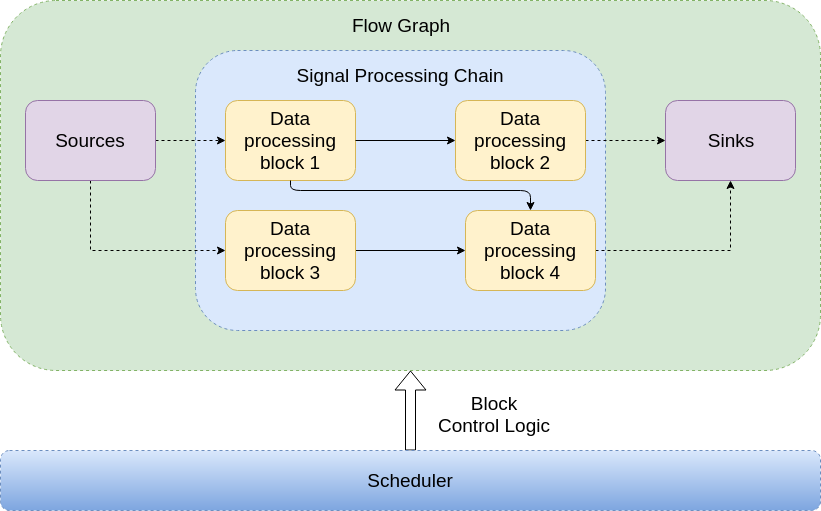
\includegraphics[width=0.9\textwidth]{Figure/GNURADIO_1.png}
\caption{GNU Radio Software Architecture.}
\label{gnuradio_arch}
\end{figure}

\paragraph{Blocks and Flow Graphs}

The computational nodes in the flow-graph are the GNU Radio processing blocks.
Each block describes how the input elements to the block, are converted to output elements in the \textit{work} function.

\begin{table}[h!]
\centering
\begin{tabular}{|c|c|c|}
\hline
Number of input elements & Number of output elements & Name\\
\hline
N & 0 & Sink Block\\
0 & N & Source Block\\
N & 1 & Interpolation block\\
1 & N & Decimation block\\
M & N & General Block\\
\hline
\end{tabular}
\caption{GNU Radio Block Types}
\label{block_type}
\end{table} 

The relationship of input and output elements defines the type of the GNU Radio processing block as shown in Table \ref{block_type}.
The type of block indicates the scheduler on how the block processes information.
There are two types of blocks: \textit{Synchronous block} and \textit{block}.
For synchronous blocks, there is a rational relationship between the input and output elements.
The sink, source, interpolation block and decimation block in Table \ref{block_type} are synchronous blocks.
The key difference between different block types is in how the scheduler handles the input and output buffers of each block.
For the synchronous blocks, the scheduler implicitly handles the input and output pointers to the buffers.
For general blocks, the \textit{work} function needs to explicitly pass the information on how many elements it consumed and produced.\\

Since in GNU Radio flow graph, data is passed from one node to another, the method of passing the data among different blocks needs to be defined.
This method is defined in the block interfaces.
Stream Interfaces are intended to stream large amounts of data between blocks with variable processing rates.
They use large buffers to pass the data from one node to another.
Stream interfaces work well for samples, bits etc. but they are not the right method to pass metadata, control information or bursts of data between blocks as it involves significant overhead.
GNU Radio recently added the message passing interface for handling asynchronous message passing.
GNU Radio also supports stream tags for handling metadata as it is closely associated with the stream data samples.
Stream tags are attached with stream data samples and provide additional information associated with the sample.
It can be used both for passing control flags as well as metadata information like the \ac{PDU} size, timing information etc.
These stream tags are propagated to the next blocks and is updated by the data rate changes.
For example, if the block takes it 2 samples as input and produces 4 samples as output, its data rate is 2.
In this case, if the input stream had a stream tag at position "x" then the the location in the output stream would be "2x". 


\begin{figure}[h!]
\centering
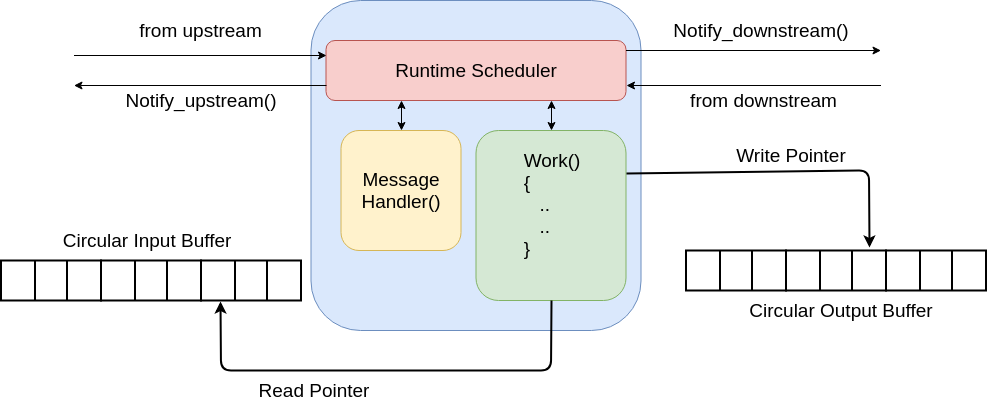
\includegraphics[width=0.9\textwidth]{Figure/Block.png}
\caption{Architecture of GNU Radio block}
\label{block_arch}
\end{figure}

Figure \ref{block_arch} shows the general architecture of a GNU Radio block. 
Each block has associated buffers for the stream interfaces, two computational components, namely the \textit{work} function and the \textit{message handler} function.
A run time scheduler is associated with each block for controlling the execution of block during runtime. The runtime scheduler has its own signaling mechanism for interacting with schedulers of other blocks.
This signaling mechanisms are hidden to the flow graph designer, and are used for flow control.
The blocks providing the inputs to the current block are called upstream blocks, while those that are fed by the output of this block are called downstream block.\\

For the sake of simplicity, it is assumed that the current block in Figure \ref{block_arch} has one upstream block and one downstream block.
This implies that the block has a single input buffer and a single output buffer.
The \textit{work} function describes the implementation of the signal processing algorithm.
On starting execution, the \textit{work} function accesses data from the circular input buffer, which is same as the output buffer for the upstream block.
Both the upstream block and the current blocks maintains a pointer to the last used data element position. 
Once completion of execution, the upstream block writes new elements to the input buffer of the current block and updates its the write data pointer.
The upstream block notifies the current block using the notify\_ downstream() method that new input data elements have been written.
The scheduler for the current block checks if there is sufficient new data for a single execution.
It then starts the execution of the current block once the input buffer has sufficient data.
On successful execution, it updates the read data pointer, writes the data elements into the output buffer and updates the write pointer.
Since, most filter design rely on history of previous inputs, the scheduler also notifies the upstream block on reading the data from the buffer to notify that its output might have been modified.
The current block scheduler notifies the downstream block that new data elements are available when it writes to the output buffer.
The \textit{message handler} function works similarly, in this case the upstream block scheduler uses notify\_msg() method for signaling that a new message may be available.\\

The flow graph describes the flow of data between different blocks.
Flow graphs make it easier to design complex signal processing algorithms by combining simpler blocks.
This provides modularity and scalability to the algorithm development process.
Generally blocks are designed in C++ to enable fine grained control and faster execution.
Python's QT framework defines a signals and slot mechanism for communicating events between different objects.
Slots are instantiation of C++ objects, which in this case are the the processing blocks.
When the internal state of the block is changed, it emits a signal which notifies other slots an event has occurred.
This mechanism is used for describing the flow graphs.


\paragraph{Scheduler}
The scheduler is the control unit for the flow graph.
At initialization, the scheduler allocates the buffers and instantiates each block in its own thread.
At runtime, it does memory management for each block, determines the requirements that are set by the block such as number of items to be processed in one execution, alignment of data in the buffers etc.
Once the requirements are satisfied, it passes the read and write pointers to the \textit{work} function and starts the one execution.
Once the \textit{work} function finishes its execution, the scheduler takes in the returned information and updates the state of the block and the appropriate pointers.\\


\section{LimeSDR-USB}
The \ac{sdr} platform used in this project is LimeSDR-USB.
It follows the architecture of the \ac{sdr} platform shown in Figure \ref{host_PHY}.
The technical specifications of LimeSDR-USB and the component description in reference to Figure \ref{host_PHY} has been summarized in Table \ref{specs}.
In the next paragraphs, the report discusses the hardware and software architecture of LimeSDR-USB.


\begin{table}[h!]
\centering
\begin{tabular}{|c|c|}
\hline
Feature & Description\\
\hline
Software Configurable RF Transreceiver & LMS7002 MIMO \ac{FPRF}\\
\ac{FPGA} & Altera Cyclone IV EP4CE40F23 \\
Bus Controller & Cypress USB 3.0 CYUSB3014-BZXC\\

\hline
\end{tabular}
\caption{LimeSDR-USB specifications}
\label{specs}
\end{table}

\subsection{LimeSDR-USB Hardware Architecture}

\begin{figure}[h!]
\centering
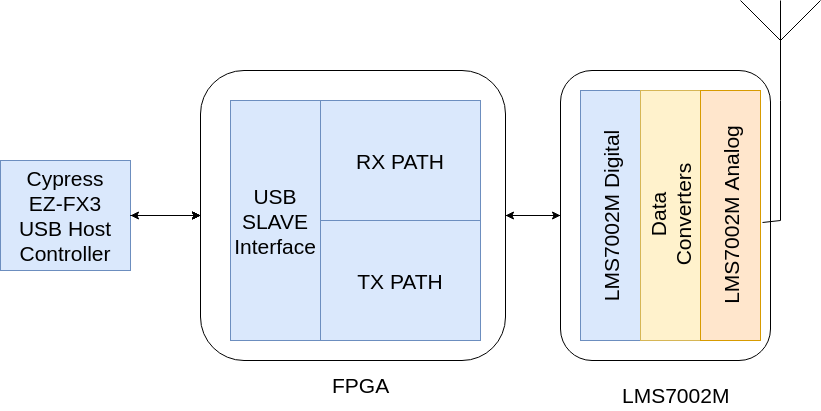
\includegraphics[width=0.9\textwidth]{Figure/Lime_Hardware.png}
\caption{Block Diagram of LimeSDR-USB.}
\label{lime_hw_arch}
\end{figure}

Figure \ref{lime_hw_arch} shows the block diagram of a LimeSDR-USB board.
For the sake of simplicity the diagram shows the major components, namely the LMS7002M \ac{FPRF}, \ac{FPGA} and the Cypress FX3 Bus Controller.
Other components will be introduced in correspondence to their application with these major components.

\paragraph{LMS7002M} 

LMS7002M is a fully intergarted \ac{FPRF} transreceiver providing 2*2 \ac{MIMO} functionality.
It provides continuous coverage of the 100kHZ- 3.8GHz frequency range, with on chip data converters providing 160 MHz \ac{RF} modulation bandwidth.
It is designed for a broad range of applications, ranging from broadband wireless communication, cellular communications, \ac{sdr} applications etc.\\
The hardware mainly consists of three main segments: analog processing chain, data converters and digital processing chain.\\

\begin{figure}[h!]
\centering
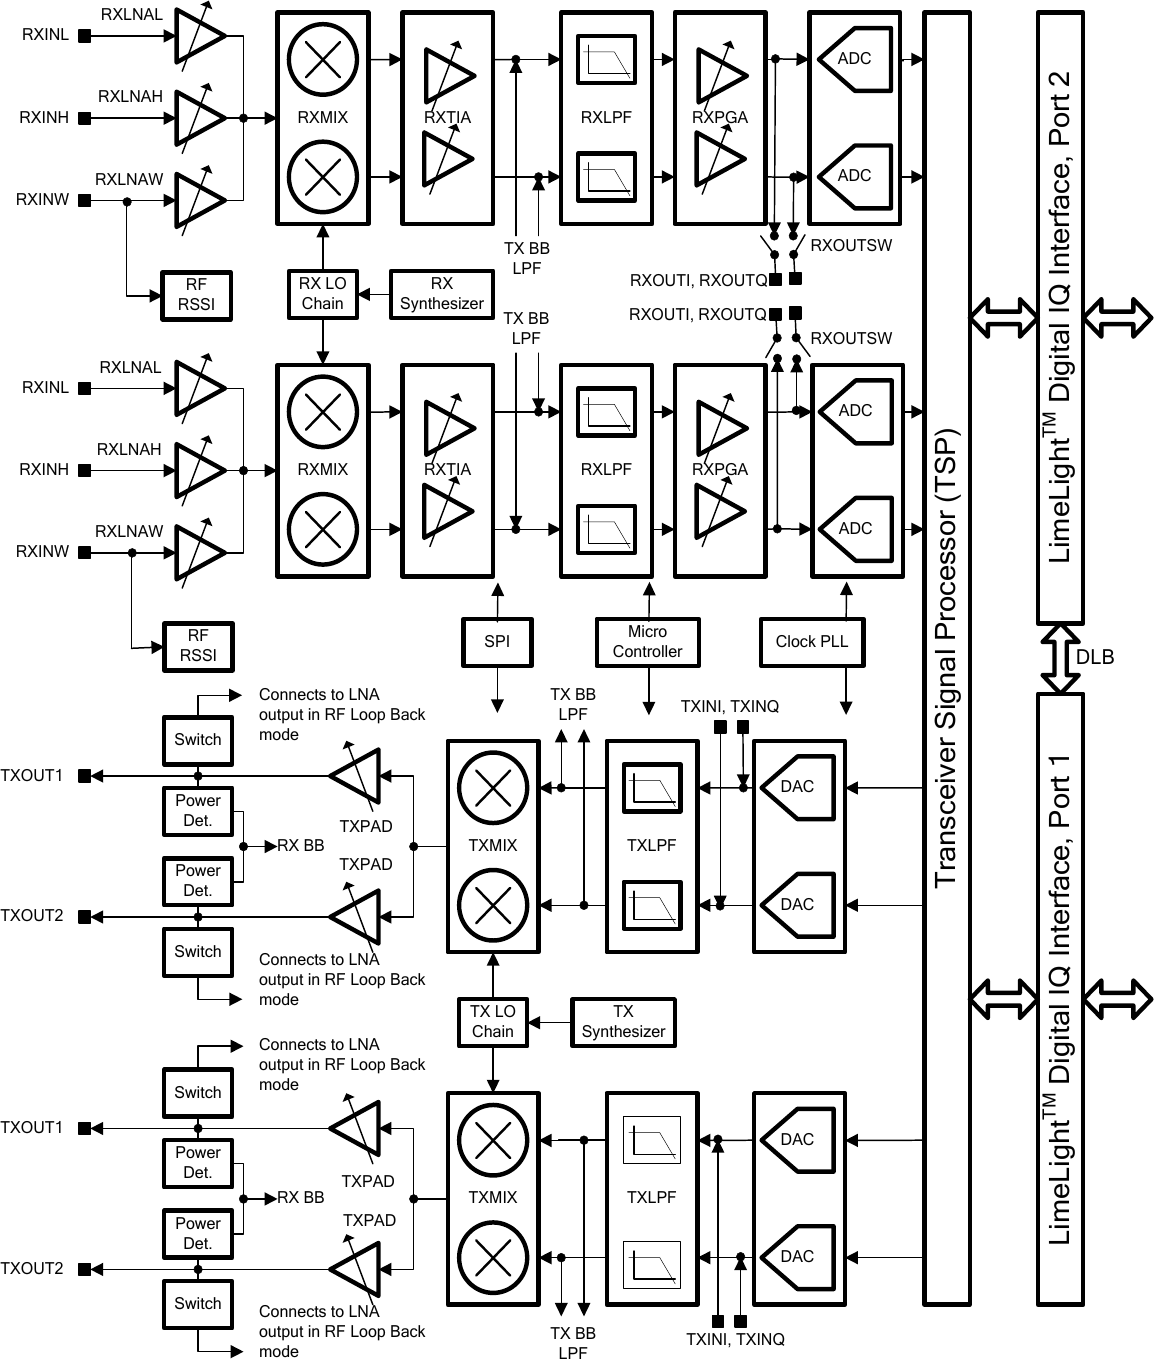
\includegraphics[width=0.9\textwidth]{Figure/Lms7002m-block-diagram.png}
\caption{Block Diagram of LMS7002M.}
\label{lms7002m}
\end{figure}

LMS7002M offers full duplex on both the TX and RX chains, enabling it to transmit and receive simultaneously.
Each of the RX chains has three separate \ac{RF} ports tuned for narrow band low frequency, narrow band high frequency and wide band operations.
Similarly, the TX Chains are connected two separate \ac{RF} ports tuned for high frequency and low frequency operations.
This separation is done for better impedance matching at the boundary of the antennas.

Figure \ref{lms7002m} shows the functional block diagram for a LMS7002M \ac{FPRF}.
Since, both the RX and TX paths are identical, the report concentrates on only one RX path.
The output from the \ac{RF} RX ports are fed into the \ac{LNA} inorder to minimize injecting too much noise at the beginning of the chain.
The receiver follows the architecture shown in Figure \ref{rf_receiver}, with a RX mixer, followed by filter and a \ac{PGA} combined in a Zero-IF architecture.
The RX \ac{PGA} outputs the analog baseband signal.\\

LMS7002M uses a fractional N-\ac{PLL} architecture for the local oscillator frequency synthesis.
\ac{PLL} is used extensively in \ac{RF} circuits for making sure the generated local oscillator signal and the reference signal have the same phase and frequency.
PLLs are essentially negative feedback systems, so when the input signal differs a lot from the output signal, the control logic tries to lower the error(\textit{input-output)}.
Integer N- \ac{PLL} architectures are used to generate high frequency signals from low frequency reference clocks, by using a frequency divider in the negative loopback path.
The frequency divider is basically a counter, that outputs every "N" (division factor of the loop) clock cycles of the output signal.
But since the output signal frequency will be multiples of the reference clock, the output signal resolution is determined by the  reference clock.
So to have a high frequency as well as a high resolution, the divider counter should be very large in size.
To counter the problem, fractional N-{PLL} architectures were designed where the output signal frequency can also be a fractional multiple of the input signal frequency.
This helps in increasing the frequency resolution without the need for a large divisor counter.
The input and output frequency relationship for a fractional  N-\ac{PLL} can be summarized by: $f_{out}=f_{ref}(N+k/M)$, where N is the integer divider factor, k is the fractional divider factor and $1/M$ gives the output frequency resolution.
Both the integer and fractional divider factor are determined by the size of the counters used.
In case of LimeSDR, the reference signal fed to the PLL varies from to 10 to 52 MHz.
The output signal can vary from 30 to 3800 MHz, with a frequency resolution of 24.8 Hz.\\

Once the \ac{RF} demodulation is completed by the analog processing chain, the analog signal is sent to the data converters and converted to digital data samples.
The sampling rate for the data conversion is determined by the \ac{RF} channel bandwidth.
The digital samples are sent to the \ac{TSP}, LMS7002M digital side, for further processing.
The \ac{TSP} uses advanced signal processing algorithms like IQ DC offset correction, IQ phase correction for correcting the received samples.
An interpolation and decimation filter is added to the \ac{TSP} for the TX and RX chains respectively.
These filters are implemented with a chain of five fixed co-efficient half band \ac{FIR} filters, which allows interpolation and decimation factors of 1,2,4,8,16.
Interpolation and Decimation allows the baseband to run at a lower data rate while still running the data converters at higher sampling rates, enabling the quantization noise to be spread over larger frequency range.
Automatic Gain Control is also implemented by the the \ac{TSP}.\\


LMS7002M interfaces can be segmented into control interfaces and data interfaces.
The control interfaces are used for initialization, calibration and on the fly reconfiguration of the LMS7002M parameters.
The data interface is used for exchanging \ac{IQ} samples with the baseband modem.
For the data interface, LMS7002M uses the LimeLight interface which implements a 12 bit JESD \ac{DDR} interface for each RX/TX chain as shown in Figure \ref{lms7002m}.
The LMS7002M has a on-chip micro-controller which can be used for configuration and control of the LMS7002M chip.
It also provides a \ac{SPI} interface for offloading the control and configuration functionality to the baseband modem.


\paragraph{FPGA}
\paragraph{Cypress FX3}

\subsection{LimeSDR USB dataflow.}
\begin{figure}[h!]
\centering
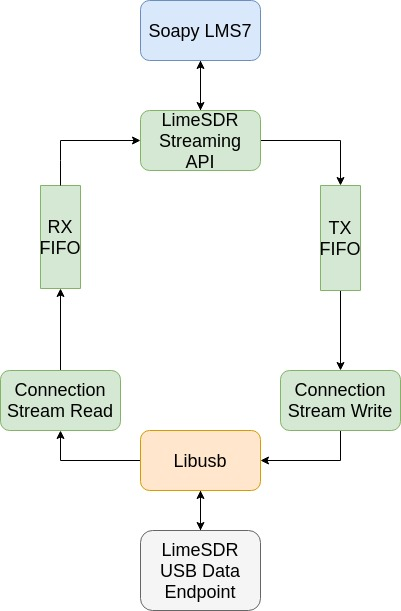
\includegraphics[scale=0.6]{Figure/Software_Architecture.jpg}
\caption{LimeSDR USB software architecture}
\end{figure}

\begin{itemize}
\item{\textit{TX Data Path:} Stream data from GNURadio is passed through Soapy drivers to the LimeSDR Streaming API. The API unwraps the data and the control flags and pushes it to the TX-FIFO. It also does the necessary data representation translation depending on the data format of the streamed data. For example, in case of complex data, it changes 32 bit I and Q value representation of GNU Radio to 16 bit I and Q values representation.  The values are pushed to the respective TX stream channel buffers(TXFIFO). The connection stream initializes the TX buffers and fills them with data from the TXFIFO. The Write function structures the data into FPGA data packet structure((Figure \ref{fpga_packet})) and combines multiple such packets into predefined batch size(initially 4). The buffer is processed by libusb to create bulk transfer packet and finally streamed to output data endpoint.}

\item{\textit{RX Data Path: } The USB data is continuously streamed from the LimeSDR to the Connection stream buffers through libusb. The Read function waits for data to be available from a usb context for the endpoint it is listening to, then it transfer data from the endpoint, parses the FPGA packets (Figure \ref{fpga_packet}) to collect the data and pushes them to the RXFIFO. If the rx stream is configured to have particular receive time, it checks if that condition is satisfied. The LimeSDR streaming API collects the data from the RXFIFO and does the necessary data interpretation translation (reverse translation to the TX Data Path), finally streams the data to GNURadio. }
\end{itemize}

\subsubsection{LimeSDR USB packets and endpoints}
LimeSDR uses four different endpoints for USB data transfer, these endpoints as Data Endpoint and Control Endpoint for both input and output directions. The control endpoints are used for configuring and retrieving data from the LMS7002M and NIOS Core on the FPGA. Data packets are used for the streaming data. 
\begin{table}[h!]
\centering
\begin{tabular}{|c|c|}
\hline
Endpoint No. & Function\\
\hline
0x01 & Stream Data Output\\
0x81 & Stream Data Input\\
0x0F & Control Data Output\\
0x8F & Control Data Input\\
\hline
\end{tabular}
\caption{LimeSDR USB transfer endpoints}
\end{table}
It uses two different packet structures for the LMS7002M Control Packets and the Stream Data Packets. Depending on the control command, different number of bytes are packed into one data element and the maximum number of blocks in a single packet is defined. One LMS64C protocol packet (Figure \ref{lms_packet}) is maximum 64 bytes, if the data to be sent is larger than that then the data field is segmented into several packets. The block count gives the number of data element in a single packet. The FPGA contains 4080 bytes of data along with 8 bytes of counter data that can be used for timestamps on the TX packets. The Lime driver uses synchronous bulk transfer for LMS Control packets and asynchronous bulk transfers for the FPGA packets.
\begin{figure}[h!]
\centering
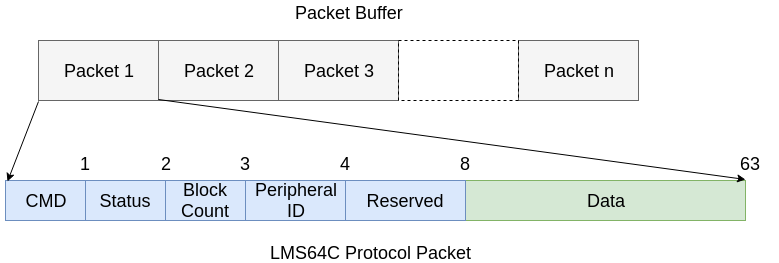
\includegraphics[width=\textwidth]{Figure/LMS64C_Packet.png}
\caption{LMS Control Packet Structure}
\label{lms_packet}
\end{figure}

\begin{figure}[h!]
\centering
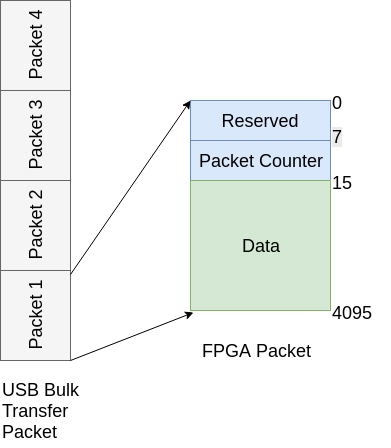
\includegraphics[scale=0.6]{Figure/FPGA_Packet.png}
\caption{FPGA Packet Structure}
\label{fpga_packet}
\end{figure}




\subsection{USBMon}
It is kernel facility provided to collect I/O traces on the USB Bus\cite{_usbmon}. USBMon reports the requests made to and by the USB Host Controller Drivers(HCD). It provides two kinds of API's : binary and character. The binary API is accessed by character devices located in the /dev namespace. The character API provides human readability and uniform format for the traces.The kernel data from the USBMon text data is made available to the userspace using debugfs\cite{_debugfs} utility.

\begin{figure}[h!]
\centering
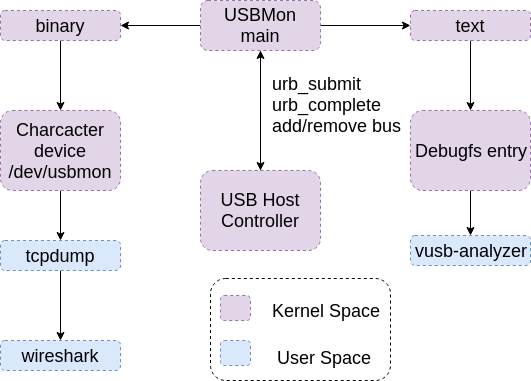
\includegraphics[width=\textwidth]{Figure/USBMon.png}
\caption{USBMon Architecture(Adapted from \cite{basak_usb_2018}).}
\end{figure}

\subsubsection{Text Data Format}
\begin{table}
\centering
\begin{tabular}{|c|c|c|c|c|}
\hline
URB Tag & Timestamp & Event Type & Address & URB Status\\
\hline
ffff8fbdbbae4000 & 2942307806 & S & Bo:3:008:15 & -115\\ 
\hline
\end{tabular}
\begin{tabular}{|c|c|c|}
\hline
Data Length & Data Tag & Data\\
\hline
64 & = & 21000100 00000000 002a0484 00000000 000000\\
\hline
\end{tabular}
\caption{Text USB Trace Example.}
\end{table}

\begin{itemize}
\item {\textit{URB Tag:} URB Identification number, it is usually the in kernel adress of the URB structure.}
\item{\textit{Timestamp:} The timestamp for the URB event at the HCD in microseconds. It is measured by the usbmon main utility using \textit{gettimeofday()} function of \textit{time.h}.}
\item{\textit{Event Type:} It specifies the event type of the HCD event. S - Submission C -Complete E - submission error.}
\item{\textit{Address: } It consists of four fields separated by colons. The URB type and direction, bus number, device number, endpoint number. The URB type and direction specifies the type of USB transfer(can be both synchronous and asynchronous).\\
\begin{table}[h!]
\centering
\begin{tabular}{|c|c|c|}
\hline
Bi & Bo & Bulk Input and Output.\\
Ci & Co & Control Input and Output.\\
Ii & Io & Interrupt Input and Output.\\
Zi & Zo & Isochronous Input and Output.\\
\hline
\end{tabular}
\caption{URB Type and Direction.}
\end{table}\\
The USB device transfers data through a pipe to a memory buffer on the host and endpoint on the device. The type of data transfer depends on the endpoint and the requirements of the function. The transfer types are as follows\cite{_usb_data_transfer}:

\begin{itemize}
\item{\textbf{Control Transfers:} It is mainly used for configuration, command and status operations.}
\item{\textbf{Bulk Transfers:} Bulk Transfer are used for bulky,non-periodic non time-sensitive burst transmissions.}
\item{\textbf{Interrupt Transfers:} It is used for mainly sending small amounts of data infrequently or asynchronously.}
\item{\textbf{Isochronous Transfers:} Isochronous transfers are mainly used for periodic, continuous streams of time sensitive data.} 
\end{itemize}
USB endpoint as explained by \cite{_usb_endpoint} , refers to the buffers on the USB device. The host computer irrespective of the host operating system can communicate by reading and writing to these buffers. They can be data endpoints and control endpoints.Data endpoints are used for transferring data whereas the control endpoint is used for configuration and device specific control.
}

\item{\textit{Data Length:} For urb\_submit it gives the requested data length and for callbacks it is the actual data length.}

\item{\textit{Data tag:} If this field is '=' then data words are present.}

\item{\textit{Data:} The data words contains in the USB transfer packet.}
\end{itemize}

\subsubsection{Raw Binary}
The overall data format is same as the text data, the data is available in raw binary by accessing character devices at /dev/usbmonX. The data can be read by using \textit{read} with \textit{ioctl} or by mapping the buffer using \textit{mmap}. The usbmon events are buffered in the following format:

\begingroup
\centering\scriptsize\begin{lstlisting}
struct usbmon_packet {
	u64 id;			/*  0: URB ID - from submission to callback */
	unsigned char type;	/*  8: Same as text; extensible. */
	unsigned char xfer_type; /*    ISO (0), Intr, Control, Bulk (3) */
	unsigned char epnum;	/*     Endpoint number and transfer direction */
	unsigned char devnum;	/*     Device address */
	u16 busnum;		/* 12: Bus number */
	char flag_setup;	/* 14: Same as text */
	char flag_data;		/* 15: Same as text; Binary zero is OK. */
	s64 ts_sec;		/* 16: gettimeofday */
	s32 ts_usec;		/* 24: gettimeofday */
	int status;		/* 28: */
	unsigned int length;	/* 32: Length of data (submitted or actual) */
	unsigned int len_cap;	/* 36: Delivered length */
	union {			/* 40: */
		unsigned char setup[SETUP_LEN];	/* Only for Control S-type */
		struct iso_rec {		/* Only for ISO */
			int error_count;
			int numdesc;
		} iso;
	} s;
	int interval;		/* 48: Only for Interrupt and ISO */
	int start_frame;	/* 52: For ISO */
	unsigned int xfer_flags; /* 56: copy of URB's transfer_flags */
	unsigned int ndesc;	/* 60: Actual number of ISO descriptors */
};	
\end{lstlisting}
\endgroup


\subsection{pidstat}
\subsection{802.15.4}
